\lab{ARMA Models}{ARMA Models}
\label{lab:arma}
\labdependencies{KalmanFilter,Pandas1}
\objective{ARMA$(p,q)$ models combine autoregressive and moving-average models in order to forecast future observations using time-series. In this lab, we will build an ARMA$(p,q)$ model to analyze and predict future weather data and then compare this model to statsmodels built-in ARMA package as well as the VARMAX package. Then we will forecast macroeconomic data as well as the future height of the Rio Negro.}

% spec file should be consistent with std and sigma...change variable to filename
% change from op.fmin to fmin
% change so its ARMA(p,q) in model identification
\section*{Time Series}


A time series is any discrete-time stochastic process.
In other words, it is a sequence of random variables, $\{Z_t\}_{t=1}^T$, that are determined by their time $t$.  We let the realization of the time series $\{Z_t\}_{t=1}^T$ be denoted by $\{z_t\}_{t=1}^T$.
Examples of time series include heart rate readings over time, pollution readings over time, stock prices at the closing of each day, and air temperature.
Often when analyzing time series, we want to forecast future data, such as what will the stock price of a company will be in a week and what will the temperature be in 10 days.

\section*{ARMA$(p,q)$ Models}

One way to forecast a time series is using an ARMA model.
The \emph{Wold Theorem} says that any covariance-stationary time series can be well approximated with an ARMA model.
An $\text{ARMA}(p,q)$ model combines an autoregressive model of order $p$ and a moving average model of order $q$ on a time series $\{Z_t\}_{t = 1}^T$.
%This model is a dependent model as it is non-independent of previous data.
%Because of this, the model needs to become stationary in order to compensate for the dependency of the data.
%To make data stationary, we look at the time series $\{z_t\}_{t=1}^T$ where $z_t=y_t-y_{t-1}$. FOR ARIMA MODELS
The model itself is a discrete-time stochastic process $(Z_t)_{t \in \mathbb{Z}}$ satisfying the equation

\begin{align}
    \label{eq:arma:def}
    Z_t = \mathbf{c} + \underbrace{\left(\sum_{i=1}^p \Phi_{i}Z_{t - i}\right)}_\text{AR(p)} +
    \underbrace{\left(\sum_{j=1}^{q} \Theta_{j} \boldsymbol{\epsilon_{t-j}} \right)}_\text{MA(q)} + \text{ }\boldsymbol{\epsilon_t}
\end{align}
where each $\boldsymbol{\epsilon_t}$ is an identically-distributed Gaussian variable with mean 0 and constant covariance $\Sigma$, \textbf{c} $\in \mathbb{R}^n$, and $\Phi_i$ and $\Theta_j$ are in $M_n(\mathbb{R})$.

\subsection*{AR($p$) Models}

An AR($p$) model works similar to a weighted random walk.
Recall that in a random walk, the current position depends on the immediate past position.
In the autogregressive model, the current data point in the time series depends on the past $p$ data points.
However, the importance of each of the past $p$ data points is not uniform.
With an error term to represent white noise and a constant term to adjust the model along the y-axis, we can model the stochastic process with the following equation:

\begin{equation}
Z_t=\mathbf{c}  + \sum_{i=1}^p\Phi_i Z_{t-i} + \boldsymbol{\epsilon_t}
\label{eq:AR}
\end{equation}

If there is a high correlation between the current and previous values of the time series, then the AR$(p)$ model is a good representation of the data, and thus the ARMA($p,q$) model will most likely be a good representation.
The coefficients $\{\Phi_i\}_{i=1}^p$ are larger when the correlation is stronger.

In this lab, we will be using weather data from Provo, Utah\footnote{This data was taken from https://forecast.weather.gov/data/obhistory/metric/KPVU.html}.
To check that the data can be represented well, we need to look at the correlation between the current and previous values.

\begin{figure}[H]
\centering
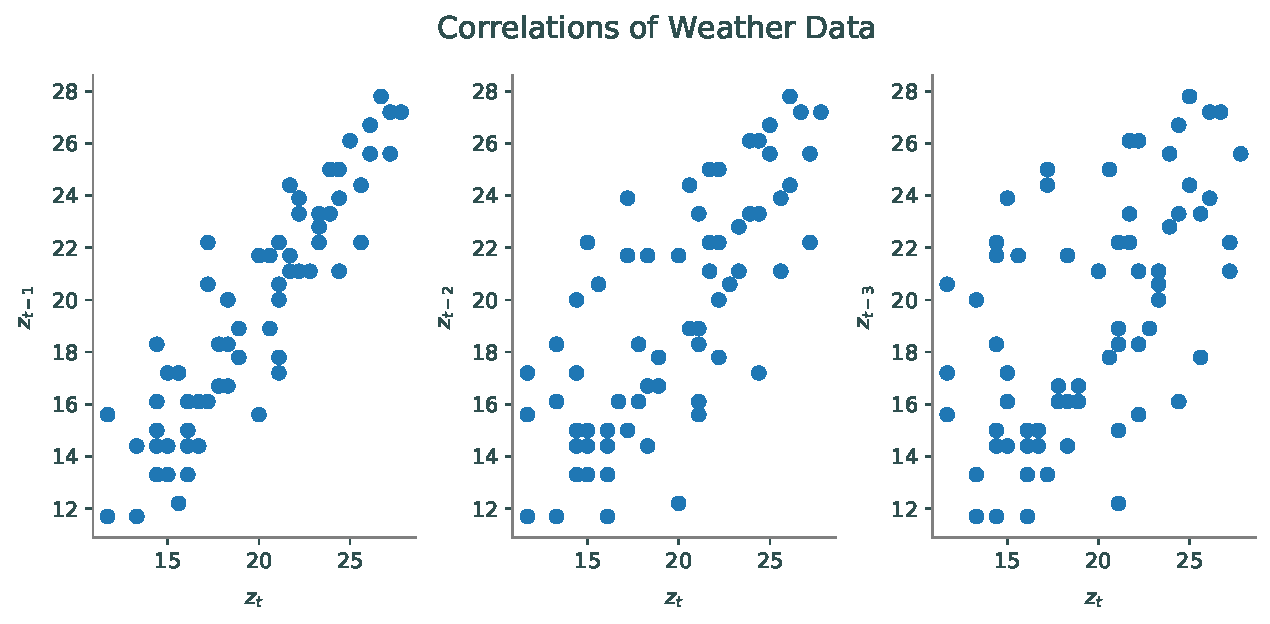
\includegraphics[width=\textwidth]{figures/correlations.pdf}
\caption{These graphs show that the weather data is correlated to its previous values.
The correlation is weaker in each graph successively, showing that the further in the past the data is, the less correlated the data becomes.}
\label{fig:correlations}
\end{figure}

\subsection*{MA($q$) Models}

A moving average model of order $q$ is used to factor in the varying error of the time series.
This model uses the error of the current data point and the previous data points to predict the next datapoint.
Similar to an AR($p$) model, this model uses a linear combination (which includes a constant term to adjust along the y-axis..

\begin{equation}
Z_t = \mathbf{c} + \boldsymbol{\epsilon_t} + \sum_{i=1}^q\Theta_i\boldsymbol{\epsilon_{t-i}}
\label{eq:MA}
\end{equation}

This part of the model simulates shock effects in the time series.
Examples of shock effects include volatility in the stock market or sudden cold fronts in the temperature.

Combining both the AR$(p$) and MA($q$) models, we get an ARMA($p,q$) model which forecasts based on previous observations and error trends in the data.

\subsection*{ARIMA$(p,d,q)$ Models}

Not all ARMA models are covariance stationary.
However, many time series can be made covariance stationary by differencing.
Let $\delta Z_t$ represent the time series $z_t = Z_t - Z_{t-1}$ obtained by taking a difference of the terms.
If the trend is linear a first difference is usually stationary.
If the trend is quadratic a second difference may be necessary $\delta ^2 Z_t = \delta ( \delta Z_t)$.
An $\text{ARIMA}(p,d,q)$ model is a discrete-time stochastic process $(Z_t)_{t \in \mathbb{Z}}$ satisfying the equation

\begin{align}
    \label{eq:arima:def}
    \delta ^ d Z_t = \mathbf{c} + \underbrace{\left(\sum_{i=1}^p \Phi_{i}z_{t - i}\right)}_\text{AR(p)} +
    \underbrace{\left(\sum_{j=1}^{q} \Theta_{j}\boldsymbol{\epsilon_{t-j}} \right)}_\text{MA(q)} + \text{ } \boldsymbol{\epsilon_t}
\end{align}


\subsection*{Finding Parameters}

One of the most difficult parts of using an ARMA($p,q$) model is identifying the proper parameters of the model.
For simplicity, at the beginning of this lab we discuss univariate ARMA models with parameters $\{\phi_i\}_{i=1}^p$, $\{\theta_i\}_{i=1}^q$, $\mu$, and $\sigma$, where $\mu$ and $\sigma$ are the mean and standard deviation of the error.
Note that $\{\phi_i\}_{i=1}^p$ and $\{\theta_i\}_{i=1}^q$ determine the order of the ARMA model.
For this lab, we will let $\mathbf{c}=0$.

A naive way to use an ARMA model is to choose $p$ and $q$ based on intuition.
Figure \ref{fig:correlations} showed that there is a strong correlation between $z_t$ and $z_{t-1}$ and between $z_t$ and $z_{t-2}$.
The correlation is weaker between $z_t$ and $z_{t-3}$.
Intuition then suggests to choose $p=2$.
By looking at the correlations between the current noise with previous noise, similar to Figure \ref{fig:correlations}, it can also be seen that there is a weak correlation between $z_t$ and $\epsilon_t$ and between $z_t$ and $\epsilon_{t-1}$.
Between $z_t$ and $\epsilon_{t-2}$ there is no correlation.
For more on how these error correlations were found, see Additional Materials.
Intuition from these correlations suggests to choose $q=1$.
Thus, a naive choice for our model is an ARMA($2,1)$ model.

\begin{figure}[H]
\centering
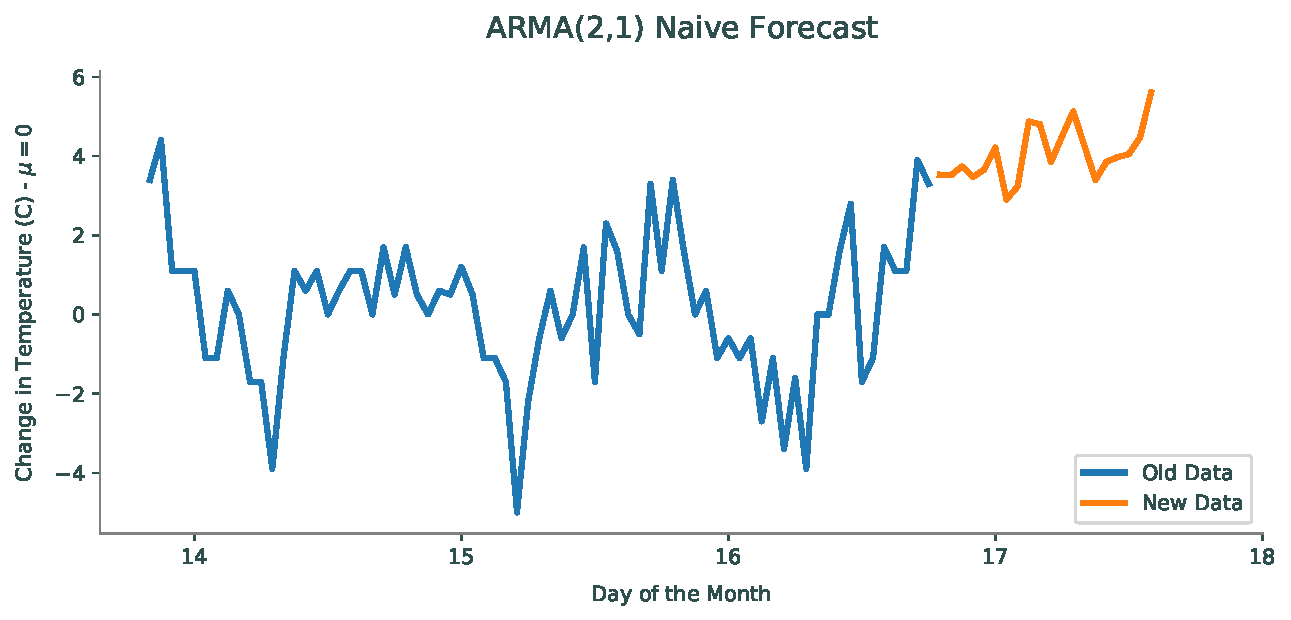
\includegraphics[width=\textwidth]{figures/naive.pdf}
\caption{Naive forecast on \li{weather.npy}}
\label{fig:ARMA:naive}
\end{figure}

\begin{problem}
Write a function \li{arma_forecast_naive()} that builds an ARMA(p,q) model.
Your function should accept as parameters \li{p}, \li{q}, and \li{n}, where \li{p} is the order of the autoregressive model, \li{q} is the order of the moving average model, and \li{n} is the number of observations to predict.
Assume \li{c}$ = 0$, and let $\phi_i=.5$, $\theta_i=.1$, and $\epsilon_i\sim\mathscr{N}(0,1)$ for all $i$.

The file \li{weather.npy} contains data on the temperature in Provo, Utah from 7:56 PM May 13, 2019 to 6:56 PM May 16, 2019, taken every hour.
This time series is NOT covariance stationary, so to make it covariance stationary, take its first difference (Hint: you might find \li{np.diff()} helpful).
We denote the new covariance stationary time series as $\{z_t\}_{t=1}^T$.
Predict the next \li{n} observations for $\{z_t\}$ by iterating through Equation \ref{eq:arima:def}.

Run your code on \li{weather.npy}, and plot the observed differences $\{z_t\}_{t=1}^T$ followed by your predicted observations of $z_t$.
For \li{p=2}, \li{q=1}, and \li{n=20}, your plot should look similar to Figure \ref{fig:ARMA:naive}, however, due to the variance of the error $\epsilon_t$, the plot will not look exactly like Figure \ref{fig:ARMA:naive}.
The predictions may be higher or lower on the $y$-axis.
\label{prob:arma:naive}
\end{problem}

Let $\Theta = \{\phi_i, \theta_j, \mu, \sigma\}$ be the set of parameters
for an $\text{ARMA}(p,q)$ model.
Suppose we have a set of observations $\{z_t\}_{t=1}^n$.
Our goal is to find the $p, q$, and $\Theta$ that maximize the likelihood of the ARMA model given the data.
Using the chain rule, we can factorize the likelihood of the model given this data as
\begin{align}
    \label{eq:arma:factorized}
    p(\{z_t\} \mid \Theta) = \prod_{t=1}^{n} p(z_t \mid z_{t-1}, \ldots, z_{1},
    \Theta)
\end{align}

\subsubsection*{State Space Representation}

In a general $\text{ARMA}(p,q)$ model, the likelihood is a function of the
unobserved error terms $\epsilon_t$ and is not trivial to compute.
Simple approximations can be made, but these may be inaccurate under certain
circumstances.
Explicit derivations of the likelihood are possible, but
tedious.
However, when the $\text{ARMA}$ model is placed in state-space, the
Kalman filter affords a straightforward, recursive way to compute the
likelihood.

We demonstrate one possible state-space representation of an $\text{ARMA}(p,q)$ model. Let
$r = \max(p,q+1)$. Define
\begin{align}
    \hat{\textbf{x}}_{t|t-1}&=\begin{bmatrix}x_{t-1}&x_{t-2}&\dotsb&x_{t-r}\end{bmatrix}\trp \\
    F &= \begin{bmatrix}
        \phi_1 & \phi_2 & \cdots & \phi_{r-1} & \phi_r\\
        1 & 0 & \cdots & 0 & 0\\
        0 & 1 & \cdots & 0 & 0\\
        \vdots & \vdots & \cdots & \vdots & \vdots\\
        0 & 0 & \cdots & 1 & 0
    \end{bmatrix}\\
    H &= \begin{bmatrix}
        1 & \theta_1 & \theta_2 & \cdots & \theta_{r-1}
    \end{bmatrix}\\
    Q &= \begin{bmatrix}
        \sigma & 0 & \cdots & 0\\
        0 & 0 & \cdots & 0\\
        \vdots & \vdots & \cdots & \vdots\\
        0 & 0 & \cdots & 0
    \end{bmatrix}\\
    w_t &\sim \text{MVN}(0, Q),
    \label{eqn:error}
\end{align}
where $\phi_i = 0$ for $i>p$, and $\theta_j = 0$ for $j > q$.
Note that Equation \ref{eq:AR} gives
\begin{align}
    F\hat{\textbf{x}}_{t-1|t-2}+w_{t}&=\begin{bmatrix}\sum_{i=1}^r\phi_ix_{t-i}\\
                                x_{t-1}\\
                                x_{t-2}\\
                                \vdots\\
                                x_{t-(r-1)}
                  \end{bmatrix}+\begin{bmatrix}\epsilon_t\\0\\0\\\vdots\\0\end{bmatrix}\\
                &=\begin{bmatrix}x_t&x_{t-1}&\cdots&x_{t-(r-1)}\end{bmatrix}\trp \\
                &=\hat{\textbf{x}}_{t|t-1}
\end{align}
We note that $z_{t|t-1}=H\hat{\textbf{x}}_{t|t-1}+\mu$.\footnote{
For a proof of this fact, see Additional Materials.}

Then the linear stochastic
dynamical system
\begin{align}
    \hat{\textbf{x}}_{t+1|t} &= F\hat{\textbf{x}}_{t|t-1} + w_t\\
    z_{t|t-1} &= H\hat{\textbf{x}}_{t|t-1} + \mu
    \label{eq:update-z}
\end{align}
describes the same process as the original $\text{ARMA}$ model.

\begin{info}
Equation \ref{eq:update-z} involves a deterministic component, namely $\mu$.
The Kalman filter theory developed in the previous lab, however, assumed $\mathbb{E}[\epsilon_t]=0$ for the observations $z_{t\mid t-1}$,.
This means you should subtract off the mean
$\mu$ of the error from the time series observations $z_{t\mid t-1}$ when using them in the predict and update
steps.
\end{info}

\subsubsection*{Likelihood via Kalman Filter}

We assumed in Equation \ref{eqn:error} that the error terms of the model are Gaussian.
This means that each conditional distribution in \ref{eq:arma:factorized} is also Gaussian, and is completely characterized by its mean and variance:
\begin{align}
    \label{eq:mean:variance1}
    \text{mean} & \quad H\hat{\textbf{x}}_{t|t-1} + \mu \\
    \label{eq:mean:variance2}
    \text{variance} & \quad HP_{t|t-1}H\trp
\end{align}
where $\hat{\textbf{x}}_{t|t-1}$ and $P_{t|t-1}$ are easily found via the Kalman filter, during the Predict step.
Given that each conditional distribution is Gaussian, the likelihood can then be found as
\begin{align}
    \label{eq:arma:likelihood}
    p(\{z_t\} \mid \Theta)& = \prod_{t=1}^{n} \mathscr{N}(z_t\mid H\hat{\textbf{x}}_{t|t-1} + \mu, HP_{t|t-1}H\trp ).
\end{align}

\begin{problem}
\label{prob:arma:likelihood}
Write a function \li{arma_likelihood()} that returns the log-likelihood of an ARMA model, given a time series $\{z_t\}_{t=1}^T$.
This function should accept \li{filename} which contains the observations, and it should accept as parameters each parameter in $\Theta$.
In this case, the time series should be the change in temperature of \li{weather.npy}, which is the first difference of the time series found in \li{weather.npy}, as was done in Problem \ref{prob:arma:naive}.
Adapt Equation \ref{eq:arma:likelihood} to calculate and return the log-likelihood of the $\text{ARMA}(p,q)$ model as a $\mathbf{float}$.

Use the provided \li{state_space_rep()} function to generate $F, Q$, and $H$.
The function \li{kalman()} has also been provided to help calculate the means and covariances of each observation.
Calling the function \li{kalman()} on a time series will return an array whose values are $\hat{\textbf{x}}_{t|t-1}$ and an array whose values are $P_{t\mid t-1}$ for each $t\leq n$.

\noindent Hint: remember to subtract off the mean $\mu$ from the inputted observation when using \li{kalman()}.

Also, when implementing Equation \ref{eq:arma:likelihood}, you may find it best to use \li{scipy.stats.distributions.norm.pdf}, but keep in mind that this method accepts standard deviations, not variances.
When implemented correctly, your function should match the following output:
\begin{lstlisting}
>>> arma_likelihood(filename="weather.npy", phis=np.array([0.9]),
                    thetas=np.array([0]), mu=17., std=0.4)
-1375.1805469978776
\end{lstlisting}
\end{problem}

\subsubsection*{Model Identification}

Now that we can compute the likelihood of a given ARMA model, we want to find the best choice of parameters given our time series.
In this lab, we define the model with the "best" choice of parameters as the model which minimizes the AIC.
The benefit of minimizing the AIC is that it rewards goodness of fit while penalizing overfitting.
The AIC is expressed by
\begin{align}
\label{eq:AIC:formula}
    2k\left(1 + \frac{k+1}{n-k}\right) - 2 \ell(\Theta)
\end{align}
where $n$ is the sample size, $k = p + q + 2$ is the number of parameters in
the model, and $\ell(\Theta)$ is the maximum likelihood for the model class.

To compute the maximum likelihood for a model class, we need to optimize
\ref{eq:arma:likelihood} over the space of parameters $\Theta$. We can do so
by using an optimization routine such as \li{scipy.optimize.minimize} on the function \li{arma_likelihood()} from Problem \ref{prob:arma:likelihood}.
Use the following code to run this routine.

\begin{lstlisting}
from scipy.optimize import minimize

# assume p, q, and time_series are defined
def f(x): # x contains the phis, thetas, mu, and std
    try:
        return -1*arma_likelihood(filename, phis=x[:i], thetas=x[i:i+j],
                                        mu=x[-2], std=x[-1])
    except np.linalg.LinAlgError:
        return np.inf

# create initial point
x0 = np.zeros(p + q + 2)
x0[-2] = time_series.mean()
x0[-1] = time_series.std()
sol = minimize(f, x0, method = "SLSQP")
sol = sol['x']
\end{lstlisting}

This routine will return a vector \li{sol} where the first $p$ values are $\{\phi_i\}_{i=1}^p$, the next $q$ values are $\{\theta_i\}_{i=1}^q$, and the last two values are $\mu$ and $\sigma$, respectively.
Note the wrapper \li{f(x)} returns the $\mathbf{negative}$ log-likelihood.
This is because \li{scipy.optimize.minimize} finds the \emph{minimizer} of $f(x)$ and we are solving for the \emph{maximum} likelihood.

To minimize the AIC, we perform \emph{model identification}.
This is choosing the order of our model, $p$ and $q$, from some admissible set.
The order of the model which minimizes the AIC is then the optimal model.

\begin{problem}
\label{prob:model-identification}
Write a function \li{model_identification()} that accepts \li{filename} containing the time series data and parameters \li{p_max} and \li{q_max} as integers.
Determine which ARMA($p,q$) model has the minimum AIC for all $1\leq p \leq \text{\li{p_max}}$ and $1\leq q \leq \text{\li{q_max}}$.
Then, return each parameter in $\Theta$ of that model.

\noindent Hint: when calculating the AIC using Equation \ref{eq:AIC:formula}, bear in mind that $-\ell(\Theta)=$ \li{f(sol)} where \li{sol} is found in the code above and explained in the following paragraph.

Your code should replicate the following output up to at least 4 decimal places.
\begin{lstlisting}
>>> model_identification(filename="weather.npy", p_max=4, q_max=4)
(array([ 0.7213538]), array([-0.26246426]), 0.359785001944352, 1.5568374351425505)
\end{lstlisting}
\end{problem}

\section*{Forecasting with Kalman Filter}
We have now identified the optimal ARMA$(p,q)$ model.
We can use this model to predict future states.
The Kalman filter provides a straightforward way to predict future states by giving the mean and variance of the conditional distribution of future observations.
Observations can be found as follows
\begin{align}
    z_{t + k} \mid z_{1}, \cdots, z_{t} \sim \mathscr{N}(z_{t+k} \mid H\hat{x}_{t+k|t} + \mu,\;
    HP_{t+k|t}H\trp )
\end{align}
To evolve the Kalman filter, recall the predict and update rules of a Kalman filter.

\begin{subequations}
    \begin{align*}
        (Initialize) \qquad \widehat{\mathbf{x}}_{0|-1} & = \boldsymbol \mu_0 \\
        \qquad P_{0|-1} & = Q_0 \\
        \vspace{0.2cm} \notag \\
        \textbf{Predict} \qquad \widehat{\mathbf{x}}_{k|k-1} & = F\widehat{\mathbf{x}}_{k-1|k-1} + \mathbf{u} && k = 1, \dots, T \\
        \qquad P_{k|k-1} & = FP_{k-1|k-1}F\trp + Q && k = 1,\dots, T \\
        \vspace{0.2cm} \notag \\
        \textbf{Update} \hspace{1.5em} \qquad K_{k} & = P_{k|k-1}H\trp \left(HP_{k|k-1}H\trp + R\right)^{-1}  && k = 0, \dots, T\\
        \qquad \widehat{\mathbf{x}}_{k|k} & = \widehat{\mathbf{x}}_{k|k-1} + K_{k}\left(\mathbf{z}_{k} - H\widehat{\mathbf{x}}_{k|k-1}\right) && k = 0, \dots, T \\
        \qquad P_{k|k} & = (I - K_{k}H)P_{k|k-1}  && k = 0, \dots, T
    \end{align*}
    \label{eqn:kalman_algorithm}
\end{subequations}

\noindent With ARMA, we define observational noise covariance $R$ and drift term $\mathbf{u}$ to both be 0.

\begin{warn}
Recall that the values returned by \li{kalman()} are conditional on the previous observation.
To compute the mean and variance of future observations, the values $x_{n|n}$ and $P_{n|n}$ MUST be computed using the Update step.
Once they are computed, only the Predict step is needed to find the future means and covariances.
\end{warn}

\begin{problem}
\label{prob:arma:forecast}
Write a function \li{arma_forecast()} that accepts \li{filename} containing a time series, the parameters for an ARMA model, and the number \li{n} of observations to forecast.
Calculate the mean and covariance of the future \li{n} observations using the Kalman filter.

To do this, use \li{state_space_rep()} to generate $F$, $Q$, and $H$.
Then, use \li{kalman()} (with $\mu$ subtracted off from the covariance stationary time series $\mathbf{z}_k$) to calculate $\hat{\mathbf{x}}_{k|k-1}$ and $P_{k|k-1}$, respectively.
Use the Update step on the last elements of $\mathbf{z}_k$ (with $\mu$ subtracted off), $\hat{\mathbf{x}}_{k|k-1}$, and $P_{k|k-1}$ to find $\hat{\mathbf{x}}_{k|k}$ and $P_{k|k}$.
Then, iteratively use the Predict step to make future predictions of the mean and covariance.
Recall that $R$ and $\mathbf{u}$ are both defined to be 0!
Also, remember that once you find a mean $\hat{\mathbf{x}}_{k|k-1}$ and covariance $P_{k|k-1}$, you must use Equations \ref{eq:mean:variance1} and \ref{eq:mean:variance2} to transform them back into observation space.

Plot the original observations as well as the mean of each future observation.
Plot a 95\% confidence interval (2 standard deviations away from the mean) around the means of future observations.
Hint: the standard deviation is the square root of the covariance calculated.

The following code should create a plot similar to Figure \ref{fig:forecasted}.

\begin{lstlisting}
# Get optimal model as found in the previous problem
phis, thetas, mu, std = np.array([0.72135856]), np.array([-0.26246788]), 0.35980339870105321, 1.5568331253098422

# Forecast optimal mode
arma_forecast(filename="weather.npy", phis=phis, thetas=thetas,
                    mu=mu, std=std, n=30)
\end{lstlisting}

\noindent How does this graph compare to the naive ARMA graph from Problem \ref{prob:arma:naive}?
\end{problem}

\section*{Statsmodel ARMA}

The module \li{statsmodels} contains a package that includes an ARMA model class.
This is accessed through ARIMA model, which stands for Autoregressive Integrated Moving Average.
This class also uses a Kalman Filter to calculate the MLE.
When creating an ARIMA object, initialize the variables \li{endog} (the data) and \li{order} (the order of the model).
The order is of the form $(p,d,q)$ where $d$ is the differences.
To create an ARMA model, set $d=0$.
The object can then be fitted based on the MLE using a Kalman Filter.

\begin{lstlisting}
from statsmodels.tsa.arima.model import ARIMA
# Intialize the object with weather data and order (1, 1)
>>> model = ARIMA(z, order=(p, 0, q), trend='c').fit(method="innovations_mle")

# Access p and q
>>> model.specification.k_ar
p
>>> model.specification.k_ma
q
\end{lstlisting}

\begin{figure}
\centering
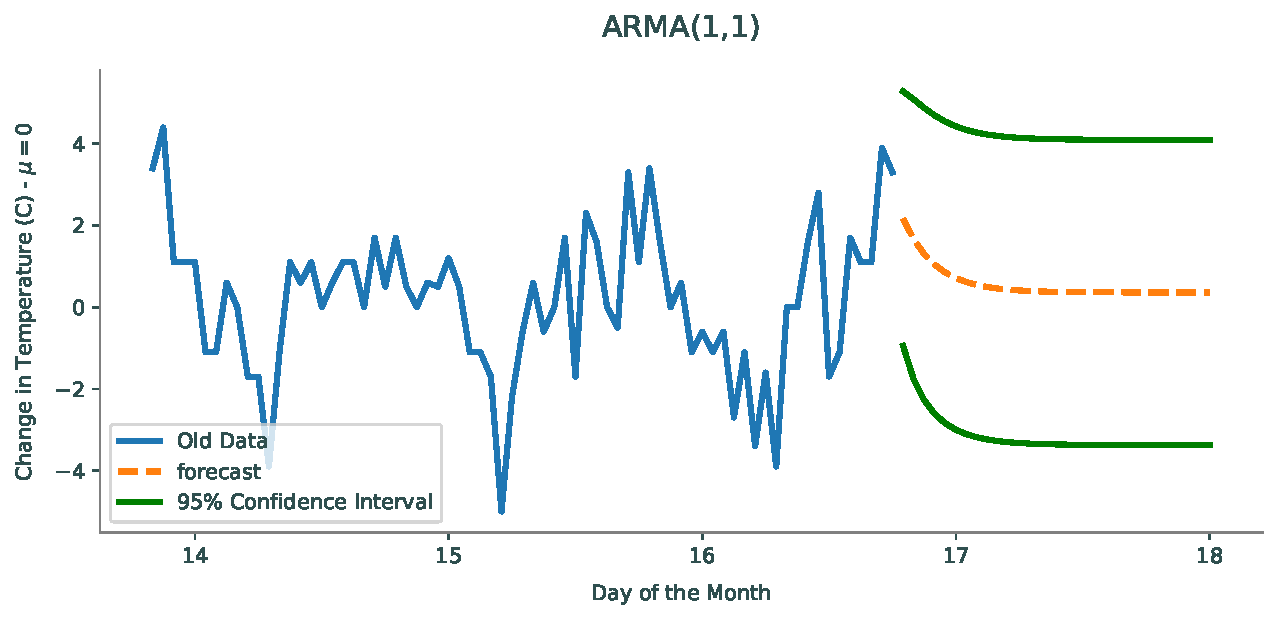
\includegraphics[width=\textwidth]{figures/arma.pdf}
\caption{ARMA(1, 1) forecast on \li{weather.npy}}
\label{fig:forecasted}
\end{figure}

As in the other problems, the time series passed in should be covariance stationary.
The AIC of an ARMA model object is saved as the attribute \li{aic}.
Since the AIC is much faster to compute using \li{statsmodels}, model identification is much faster.
Once a model is chosen, the method \li{predict} will forecast $n$ observations, where $n$ is the number of known observations.
It will return the mean of each future observation.

\begin{lstlisting}
# Predict from the beginning of the model to 30 observations in the future
model.predict(start=0, end=len(data)+30)
\end{lstlisting}

\begin{problem}
Write a function \li{sm_arma()} that accepts \li{filename} containing a time series, integer values for \li{p\_max} and \li{q\_max}, and the number \li{n} of values to predict.

As in Problem \ref{prob:model-identification}, perform model identification to find the ARMA($p,q$) model with the best AIC for $1\leq p \leq$ \li{p_max} and $1 \leq q \leq$ \li{q_max}, but this time use \li{statsmodels}.
Make sure the model is fit using the MLE.

Use the optimal model to predict \li{n} future observations of the time series.
Plot the original observations along with the predicted observations from the beginning through \li{n} observations in the future, as given by \li{statsmodels}.
\textbf{Return the AIC} of the optimal model.

For \li{p\_max=3}, \li{q\_max=3}, and \li{n=30}, your graph should look similar to Figure \ref{fig:sm}.
How does this graph compare to Problem \ref{prob:arma:naive}? Problem \ref{prob:arma:forecast}?
\label{prob:statsmodels}
\end{problem}

\begin{figure}[H]
\centering
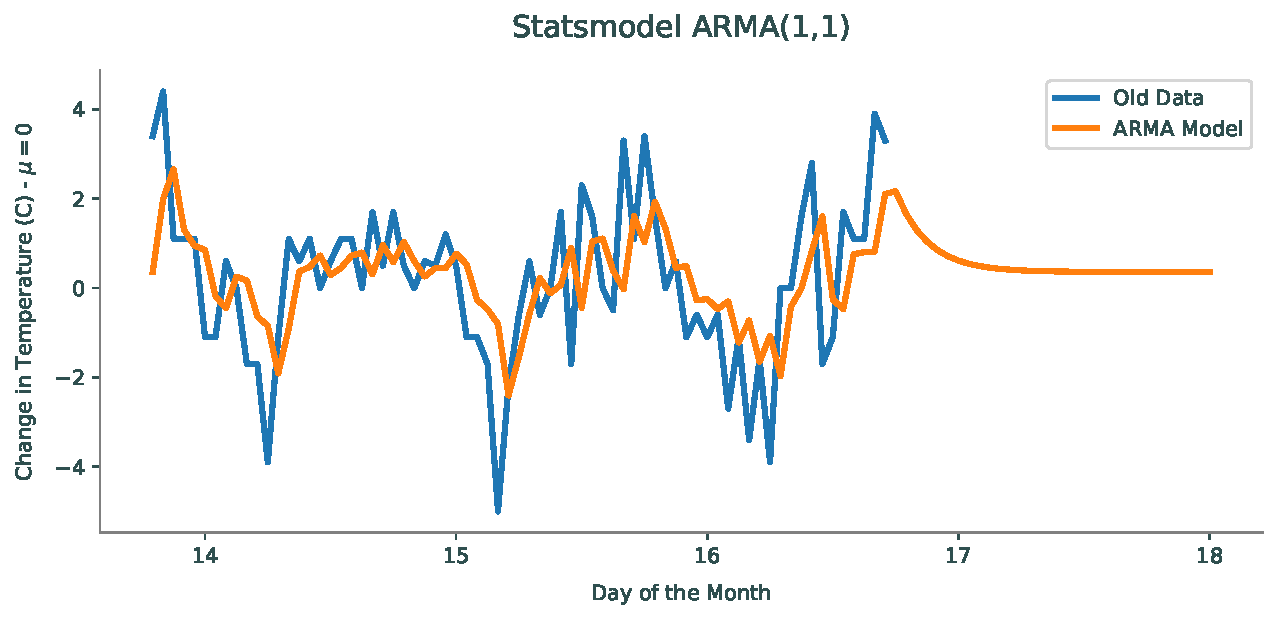
\includegraphics[width=\textwidth]{figures/sm.pdf}
\caption{Statsmodel forecast on \li{weather.npy}.}
\label{fig:sm}
\end{figure}


\section*{Statsmodel VARMA}
Until now we have been dealing with univariate ARMA models.
Multivariate ARMA models are used when we have multiple time series that can be useful in predicting one another.
For example say we have two time series $z_{t,1}$ and $z_{t,2}$.
The multivariate ARMA(1,1) model is as follows:

\begin{align}
	z_{t,1} = c_1 + \phi_{11} z_{t-1,1} +  \phi_{12} z_{t-1,2} +  \theta_{11} \epsilon_{t-1,1} +  \theta_{12} \epsilon_{t-1,2}
	\\
	z_{t,2} = c_1 + \phi_{21} z_{t-1,1} +  \phi_{22} z_{t-1,2} +  \theta_{21} \epsilon_{t-1,1} +  \theta_{22} \epsilon_{t-1,2}
\end{align}

This can be written in matrix form as shown in Equation \ref{eq:arma:def}.
The module \li{statsmodels} contains a package that includes a VARMAX model class which can be used to create a multivariate ARMA model.
VARMAX stands for Vector Autoregression Moving Average with Exogenous Regressors.
An exogenous regressor is a time series that affects the model but is not affected by it.
In the example below we have two time series corresponding to the price of copper and aluminum.
Since aluminum is a substitute for copper, it is reasonable to assume the price of aluminum may help us predict the price of copper and vice versa.

\begin{lstlisting}
from statsmodels.tsa.api import VARMAX
import statsmodels.api as sm

# Load in world copper data
data = sm.datasets.copper.load_pandas().data
# Create index compatible with VARMAX model
data.index = pd.period_range(start="1951", end="1975", freq='Y')

# Initialize and fit model
mod = VARMAX(data[["ALUMPRICE", "COPPERPRICE"]])
mod = mod.fit(maxiter=1000, disp=False)
# Predict the price of aluminium and copper until 1985
pred = mod.predict("1951", "1985")

# Get confidence intervals
forecast_obj = mod.get_forecast("1981")
all_CI = forecast_obj.conf_int(alpha=0.05)

# Plot predictions against true price
pred.plot(figsize=(10,4))
plt.plot(data["ALUMPRICE"], label="Actual ALUMPRICE")
plt.plot(data["COPPERPRICE"], label="Actual COPPERPRICE")
plt.legend()
plt.title("VARMA Predictions for World Copper Market Dataset")
\end{lstlisting}

\begin{figure}[H]
\centering
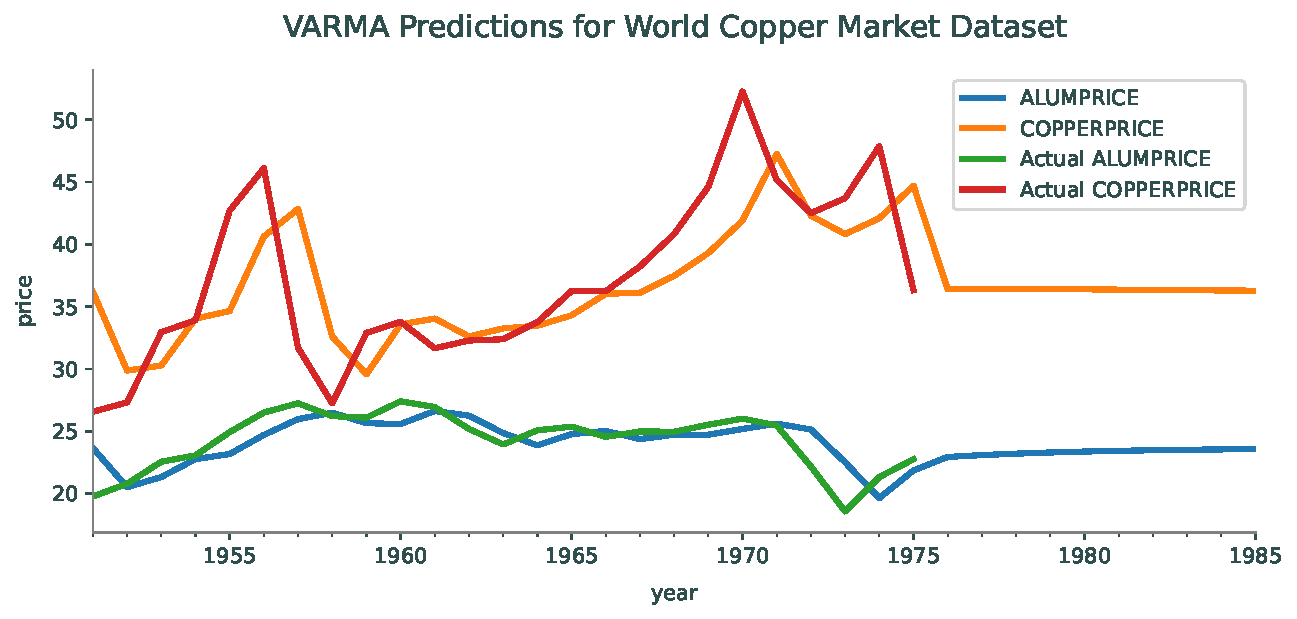
\includegraphics[width=\textwidth]{figures/copper.pdf}
\caption{Statsmodel VAR(1) forecast.}
\label{fig:varma}
\end{figure}

\begin{problem}
\label{prob:arma:smvarma}

Write a function \li{sm_varma()} that accepts start and end dates for forecasting.
Use the statsmodels VARMAX class to forecast on macroeconomic data between the start and end dates.
The following code shows how to obtain the data.

\begin{lstlisting}
# Load in data
df = sm.datasets.macrodata.load_pandas().data
# Create DatetimeIndex
dates = df[["year", "quarter"]].astype(int).astype(str)
dates = dates["year"] + "Q" + dates["quarter"]
dates = dates_from_str(dates)
df.index = pd.DatetimeIndex(dates)
# Select columns used in prediction
df = df[["realgdp", "realcons", "realinv"]]
\end{lstlisting}

Initialize your VARMAX model with the \li{df} specified above, and include the parameter \li{freq="Q-DEC"}.
Fit your model, and predict from the start date until the end date.
Then, get the model forecast until the end date.
Plot the original data, prediction, and a 95\% confidence interval (2 standard deviations away from the mean) around the future observations.
\textbf{Return the AIC} of the chosen model.
The plot should be similar to Figure \ref{fig:econ}.

\noindent Hint: in the example above, \li{mod.predict("1951", "1985")} returns a dataframe of 2 columns that contain the predicted values of \li{"ALUMPRICE"} and \li{"COPPERPRICE"}, respectively, from the years 1951 to 1985.
Also, \li{all_CI} is a dataframe where each column indicates the corresponding dataset and whether it is a lower or upper bound of a confidence interval determined by the alpha value.
Thus, the column \li{"lower ALUMPRICE"} with \li{alpha=0.05} contains the lower bounds of a 95\% confidence interval for the \li{"ALUMPRICE"} dataset.

The dataset \li{"realgdp"} contains the real gross domestic product, \li{"realcons"} contains real personal consumption expenditures, and \li{"realinv"} contains real gross private domestic investment.
Since personal consumption and domestic investment are components of gross domestic product, it is reasonable to assume these time series will be useful in predicting one another.

\end{problem}

\begin{figure}[H]
\centering
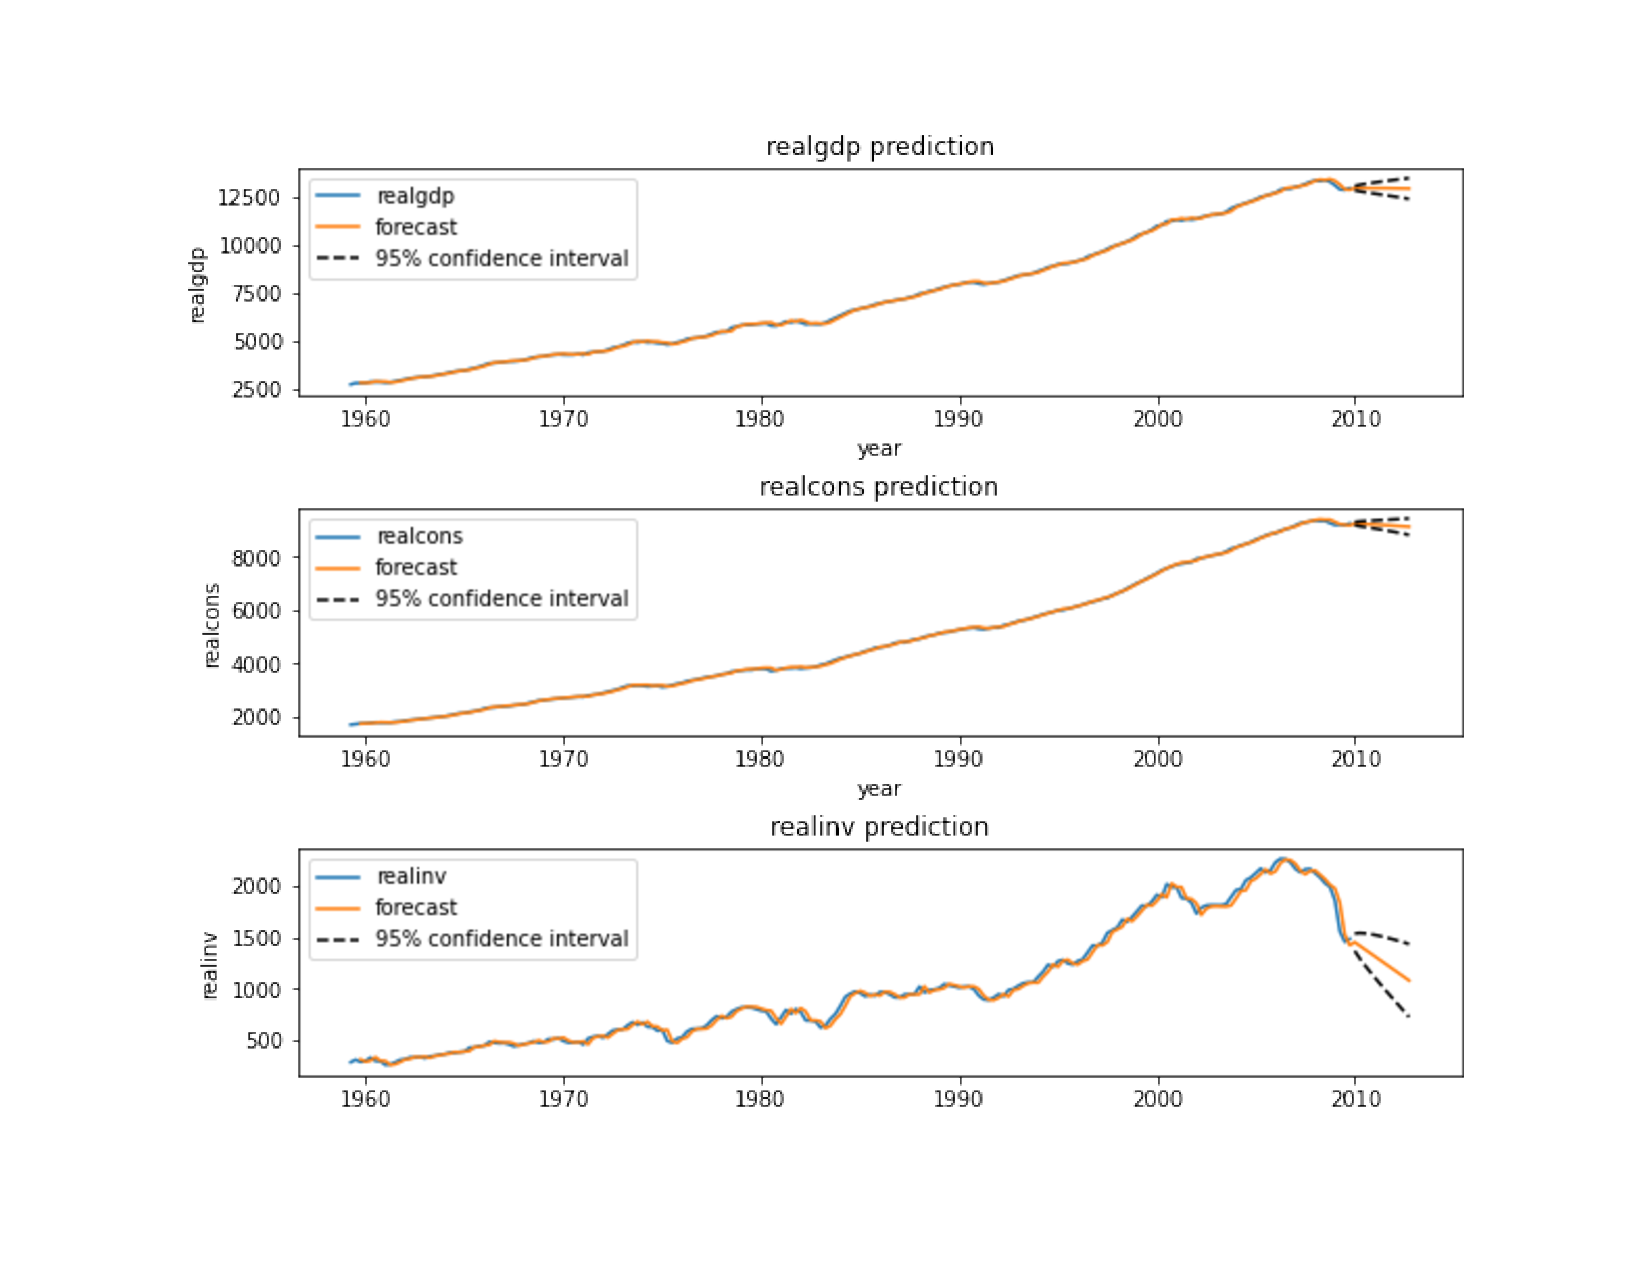
\includegraphics[width=\textwidth]{figures/econ2.pdf}
\caption{Macroeconomic data is forecasted 12 years in the future using statsmodels.}
\label{fig:econ}
\end{figure}

\section*{Optional}
%In the previous problem, we used the statsmodel \li{ARIMA} class.
%The following code and problem use the soon to be depreciated \li{ARMA} class
The \li{statsmodels} package can help us perform model identification.
The method \li{arma_order_select_ic} will find the optimal order of the ARMA model based on certain criteria.
The first parameter \li{y} is the data.
The data must be a NumPy array, not a Pandas DataFrame.
The parameter \li{ic} defines the criteria trying to be minimized.
The method will return a dictionary, where the minimal order of each criteria can be accessed.
%\footnote{http://www.statsmodels.org/devel/generated/statsmodels.tsa.stattools.arma_order_select_ic.html}.

\begin{lstlisting}
>>> import statsmodels.api as sm
>>> from statsmodel.tsa.stattools import arma_order_select_ic as order_select
>>> import pandas as pd

>>> # Get sunspot data and give DateTimeIndex
>>> sunspot = sm.datasets.sunspots.load_pandas().data
>>> sunspot.index = pd.Index(pd.date_range("1700", end="2009", freq="A-DEC"))
>>> sunspot.drop(columns = ["YEAR"],inplace = True)

>>> # Find best order where p < 5 and q < 5
>>> # Use AICc as basis for minimization
>>> order = order_select(sunspot.values,max_ar=4,max_ma=4,ic=["aic", "bic"],fit_kw={"method": "mle"})
>>> print(order["aic_min_order"])
(4,2)
>>> print(order["bic_min_order"])
(4,2)

>>> # Fit model
>>> # Note that we need to set the dimensionality to zero in order to have an ARMA model.
>>> model = ARIMA(sunspot,order = (4,0,2)).fit(method="innovations_mle")

>>> # Predict values from 1950 to 2012.
>>> prediction = model.predict(start="1950", end="2012")

>>> # Plot the prediction along with the sunspot data.
>>> fig, ax = plt.subplots(figsize=(13, 7))
>>> plt.plot(prediction)
>>> plt.plot(sunspot["1950": "2009"])
>>> ax.set_title("Sunspot Dataset")
>>> ax.set_xlabel("Year")
>>> ax.set_ylabel("Number of Sunspots")
>>> plt.show()
\end{lstlisting}

%The method \li{plot_predict} accepts a time series and plots the ARMA model alongside the original data in a given range.
%The plot of the ARMA model is the mean calculated by ARMA at each data point, both known and future.
%This method works by giving a range on which to plot the ARMA model.
%This range can be given by indices (as in Problem \ref{prob:statsmodels}) or by a DateTimeIndex.

\begin{figure}[H]
\centering
\includegraphics[width=\textwidth]{figures/sunspot.pdf}
\caption{Sunspot activity data is forecasted four years in the future using \li{statsmodels.}}
\label{fig:sunspot}
\end{figure}

\begin{problem}
The dataset \li{manaus} contains data on the height of the Rio Negro from every month between January 1903 and January 1993.
Write a function \li{manaus()} that accepts the forecasting range as strings \li{start} and \li{end}, the maximum parameter for the AR model \li{p} and the maximum parameter of the MA model \li{q}.
The parameters \li{start} and \li{end} should be strings corresponding to a DateTimeIndex in the form \li{Y\%M\%D}, where \li{D} is the last day of the month.

The function should determine the optimal order for the ARMA model based on the AIC and the BIC.
Then forecast and plot on the range given for both models and compare.
Return the order of the AIC model and the order of the BIC model, respectively.
For the range \li{"1983-01-31"} to \li{"1995-01-31"}, your plot should look like Figure \ref{fig:manaus}.

(Hint: The data passed into \li{arma_order_select_ic} must be a NumPy array. Use the attribute \li{values} of the Pandas DataFrame.)

To get the \li{manaus} dataset and set it with a DateTimeIndex, use the following code:
\begin{lstlisting}
# Get dataset
raw = pydata("manaus")
# Convert to DateTimeIndex
manaus = pd.DataFrame(raw.values,index=pd.date_range("1903-01", "1993-01", freq='M'))
manaus = manaus.drop(0, axis=1)
# Set new column title
manaus.columns = ["Water Level"]
\end{lstlisting}
\label{prob:manaus}
\end{problem}

\begin{figure}[H]
\centering
\includegraphics[width=\textwidth]{figures/manaus.pdf}
\caption{AIC and BIC based ARMA models of \li{manaus} dataset.}
\label{fig:manaus}
\end{figure}

% Additional Materials

\pagebreak

\section*{Additional Materials}

\subsection*{Finding Error Correlation}
To find the correlation of the current error with past error, the noise of the data needs to be isolated.
Each data point $y_t$ can be decomposed as

\begin{equation}
y_t=T_t+S_t+R_t,
\end{equation}

where $T_t$ is the overall trend of the data, $S_t$ is a seasonal trend, and $R_t$ is noise in the data.
The overall trend is what the data tends to do as a whole, while the seasonal trend is what the data does repeatedly.
For example, if looking at airfare prices over a decade, the overall trend of the data might be increasing due to inflation.
However, we can break this data into individual years.
We call each year a season.
The seasonal trend of the data might not be strictly increasing, but have increases during busy seasons such as Christmas and summer vacations.

To find $T_t$, we use an $M$-fold method.
In this case, $M$ is the length of our season.
We define the equation

\begin{equation}
T_t=\frac{1}{M}\sum_{-M/2<i<M/2}y_{i+t}.
\end{equation}

This means for each $t$, we take the average of the season surrounding $y_t$.

To find the seasonal trend, first subtract the overall trend from the time series.
Define $x_t=y_t-T_t$.
The value of the seasonal trend can then be found by averaging each day of the season over every season.
For example, if the season was one year, we would find the average value on the first day of the year over all seasons, then the second, and so on.
Thus,

\begin{equation}
S_t=\frac{1}{K}\sum_{i\equiv t\text{ (mod $M$)}}x_i
\end{equation}
where $K$ is the number of seasons.

With the overall and seasonal trend known, the noise of the data is simply $R_t=y_t-T_t-S_t$.
To determine the strength of correlations with the current error and the past error, plot $y_t$ vs. $R_{t-i}$ as in Figure \ref{fig:correlations}.

\subsection*{Proof of Equation \ref{eq:update-z}}
\begin{align}
    \sum_{i=1}^p\phi_i(z_{t-i}-\mu)+a_t+\sum_{j=1}^q\theta_ja_{t-j}&=\sum_{i=1}^p\phi_i(H\hat{\textbf{x}}_{t-i})+a_t+\sum_{j=1}^q\theta_ja_{t-j}\\
    &=\sum_{i=1}^r\phi_i(x_{t-i}+\sum_{k=1}^{r-1}\theta_kx_{t-i-k})+a_t+\sum_{j=1}^{r-1}\theta_ja_{t-j}\\
    &=a_t+\sum_{i=1}^r\phi_i(x_{t-i})+\sum_{j=1}^{r-1}\theta_j\Bigl(\sum_{i=1}^r\phi_ix_{t-j-i}+a_{t-j}\Bigr)\\
    &=a_t+\sum_{i=1}^r\phi_i(x_{t-i})+\sum_{j=1}^{r-1}\theta_jx_{t-k}\\
    &=x_t+\sum_{j=1}^{r-1}\theta_jx_{t-k}\theta_kx_{t-k}\\
    &=z_t.
\end{align}

%%%%%%%%%%%%%%%%%%%%%%%%%%%%%%%%%%%%%%
